%
% Chapter 7
%
\chapter {Trapped-Ions Physical Platform}

Trapped ions is one of the most promising approaches to the physical implementation of a quantum computer\cite{TrappedIonQuantumComputing_2019}. The basic requirements for a universal quantum computer, as outlined by David DiVicenzo\cite{ThePhysicalImplementationOfQuantumComputation_DiVicenzo_2000}, have been demostrated with trapped ions, and a few companies are using this approach to build their quantum computers (e.g. IonQ \cite{IonQTechnology}, Honeywell \cite{HoneywellSystemModelH1}).

\section{Platform Characteristics}

In this physical platform, qubits are ions confined and suspended in free space using electromagnetic fields, and its internal electronic states are used as qubit states $\ket{0}$ and $\ket{1}$. Initialization of the qubits is performed by laser manipulation. State $\ket{0}$ is a long-lived ground state and state $\ket{1}$ can be prepared by optically pumping the ion to an auxiliary state $\ket{e}_{SP}$ that rapidly decays into state $\ket{1}$ as shown in figure \ref{fig:QubitInitialization}.

\begin{figure}[h!]
    \centering
    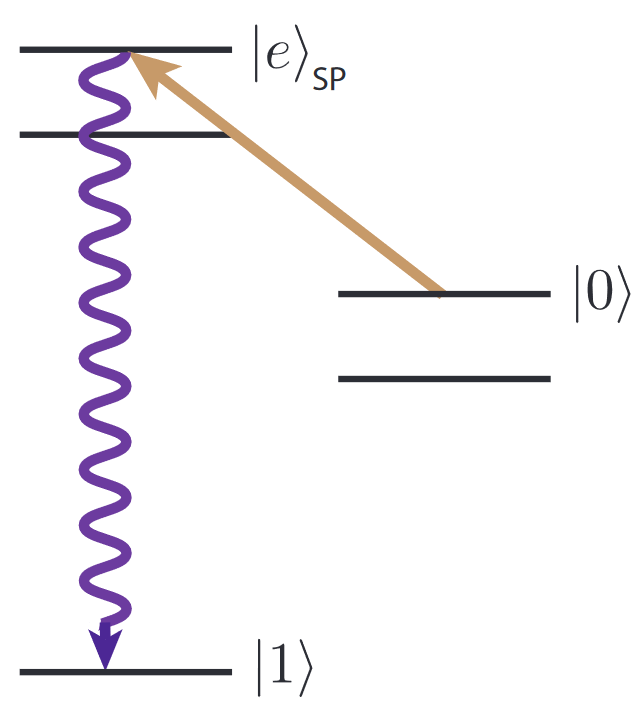
\includegraphics[scale=.30]{images/TrappedIons-StatePreparation.png}
    \caption{Qubit initialization \cite{TrappedIonQuantumComputing_2019}}
    \label{fig:QubitInitialization}
\end{figure}

As shown in figure \ref{fig:QubitReadout}, qubit readout is done by using a resonant laser that couples the $\ket{1}$ state to a $\ket{e}_{R}$ state which scatters many photons that can be collected by a detector. When the ion is in state $\ket{0}$, it does not interact with the laser so no photons are emitted and the image produced by the detector is dark.

\begin{figure}[h!]
    \centering
    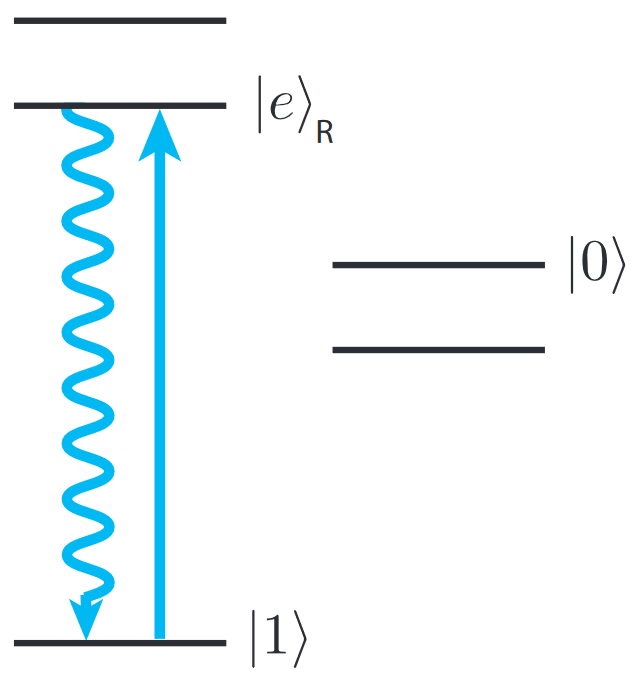
\includegraphics[scale=.25]{images/TrappedIons-QubitReadout.png}
    \caption{Qubit readout \cite{TrappedIonQuantumComputing_2019}}
    \label{fig:QubitReadout}
\end{figure}

A universal gate set is achieved by providing two qubit manipulation mechanisms:
\begin{itemize}[noitemsep,nolistsep]
    \item Arbitrary single qubit rotations: laser or microwave drives applied to the ions allow arbitrary and high fidelity single qubit rotations to be performed.
    \item An entangling operation: motional modes of two or more ions are used as a bus for transfering quantum information among ions.
\end{itemize}

Single qubit gate times are in the order of a few microseconds while two qubit gate times typically take between tens and hundreds of microseconds. Ion coherence times range from 0.2 seconds in optical qubits to up to 600 seconds for hyperfine qubits. Long coherence times relative to gate times fulfill the remaining criteria for a universal quantum computer.

\section{Native Gates}

The native single qubit gate\cite{3QubitGroverSearch_2017} in this physical platform is defined as:
$$R(\theta,\phi)=\left[\begin{array}{cc}\cos{\frac{\theta}{2}} & -\imath e^{-\imath \phi}\sin{\frac{\theta}{2}} \\ -\imath e^{-\imath \phi}\sin{\frac{\theta}{2}} & \cos{\frac{\theta}{2}}\end{array}\right]$$

Rotations about the X-axis ($R_x(\theta)$) are achieved by setting $\phi=0$. Rotations about the Y-axis ($R_y(\theta)$) are achieved by setting $\phi=\frac{\pi}{2}$. Rotations about the Z-axis ($R_z(\theta)$) are achieved by three rotations about axes in the XY plane as shown in figure \ref{fig:RzGate}:

\begin{figure}[h!]
    \centering
    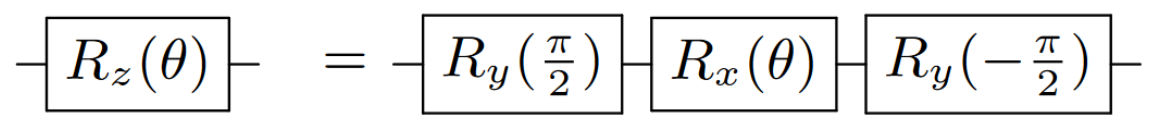
\includegraphics[scale=.35]{images/TrappedIons-RzGate.png}
    \caption{Rz gate \cite{3QubitGroverSearch_2017} decomposition}
    \label{fig:RzGate}
\end{figure}

Note that Pauli gates can be constructed from rotations around the X, Y and Z axis:
\begin{itemize}[noitemsep,nolistsep]
    \item $X=\imath R_x(\pi)$
    \item $Y=\imath R_y(\pi)$
    \item $Z=\imath R_z(\pi)$
\end{itemize}

Another widely used quantum gate is the Hadamard gate, which can be also be decomposed from rotations around the X and Y axis\cite{QuantumInspire_HadamardGate}:
$$H=R_x(\pi)R_y(\frac{\pi}{2})$$

The native two qubit entangling gate\cite{3QubitGroverSearch_2017} in this physical platform is defined as:
$$XX(\chi)=\left[\begin{array}{cccc}\cos{\chi} & 0 & 0 & -\imath\sin{\chi} \\ 0 & \cos{\chi} & -\imath\sin{\chi} & 0 \\ 0 & -\imath\sin{\chi} & cos{\chi} & 0 \\ -\imath\sin{\chi} & 0 & 0 & cos{\chi}\end{array}\right]$$

The CNOT gate, which is more commonly used as an entangling gate when describing quantum algorithms, can be constructed using the $XX(\chi)$ and $R(\theta,\phi)$ gates as shown in figure \ref{fig:CNOTGate}:

\begin{figure}[h!]
    \centering
    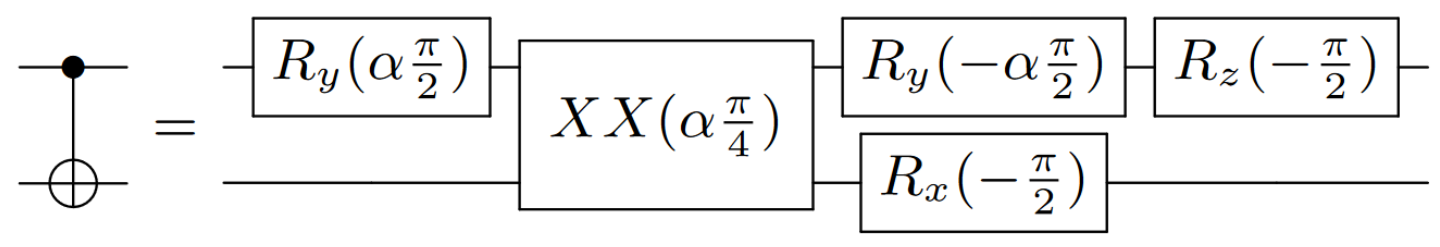
\includegraphics[scale=.35]{images/TrappedIons-CNOTGate.png}
    \caption{CNOT gate \cite{3QubitGroverSearch_2017} decomposition where $\alpha=sgn(\chi)$}
    \label{fig:CNOTGate}
\end{figure}

Using the results demonstrated by C. J. Ballance et al. \cite{TrappedIonHyperfineQubits_2016}, the gate times and fidelities in this physical platform are the following:
\begin{itemize}[noitemsep,nolistsep]
    \item Single qubit arbitrary rotation gate ($R(\theta,\phi)$):
    \begin{itemize}[noitemsep,nolistsep]
        \item Time: 7.5 $\mu s$
        \item Fidelity: 0.99993
    \end{itemize}
    \item Two qubit entangling gate ($XX(\chi)$): .
    \begin{itemize}[noitemsep,nolistsep]
        \item Time: 100 $\mu s$
        \item Fidelity: 0.999
    \end{itemize}
\end{itemize}

\section{Resources Estimation Analysis}

\todo{Show (using tables and/or plots) how resources escalate as the size and pattern of the input changes}.

\section{Analysis of Execution in NISQ Devices}

\todo{Analyze what would be the maximum input size that can be successfully run on a NISQ device based on this platform.}

\section{Analysis of Execution of Algorithm for Input of Specific Size}

\todo{Use a resource estimator to determine the characteristics that a device should have to run the algorithm for a specific input size, and determine what would be the runtime.}
